% !TeX TXS-program:bibliography = txs:///biber
\documentclass[fontsize=14pt, russian]{scrartcl}
\input{header.tex}
\addbibresource{biblio.bib}

\usepackage{svg}
    
\begin{document}
\sloppy

\def\figurename{Рисунок}

\begin{titlepage}
    \thispagestyle{empty}
    \newpage

    \bmstuheader

    \vspace{3em}

    \begin{center}
        {\Large\bfseries РАСЧЕТНО-ПОЯСНИТЕЛЬНАЯ ЗАПИСКА\\\textbf{\textit{К НАУЧНО-ИССЛЕДОВАТЕЛЬСКОЙ РАБОТЕ\\НА ТЕМУ:}} \\}
    \end{center}

    \vspace*{-6ex}
    \begin{center}
        \Large{\textit{\textbf{}}}

        \vspace*{-3ex}
        \rule{1\textwidth}{1.2pt}

        \vspace*{-0.2ex}

        \Large{\textit{\textbf{}}}

        \vspace*{-3ex}
        \rule{1\textwidth}{1.2pt}

        \vspace*{-0.2ex}
        \rule{1\textwidth}{1.2pt}

        \vspace*{-0.2ex}
        \rule{1\textwidth}{1.2pt}
    \end{center}

    \vspace{\fill}


    \newlength{\ML}
    \settowidth{\ML}{«\underline{\hspace{0.7cm}}» \underline{\hspace{2cm}}}

    \noindent Студент \underline{\hspace{1.5cm}} \hfill \underline{\hspace{4cm}}\quad
    \underline{\hspace{4cm}}

    \vspace{-2.1ex}
    \noindent\hspace{9ex}\scriptsize{(Группа)}\normalsize\hspace{170pt}\hspace{2ex}\scriptsize{(Подпись, дата)}\normalsize\hspace{30pt}\hspace{6ex}\scriptsize{(И.О. Фамилия)}\normalsize

    \bigskip

    \noindent Руководитель НИР \hfill \underline{\hspace{4cm}}\quad
    \underline{\hspace{4cm}}

    \vspace{-2ex}
    \noindent\hspace{13.5ex}\normalsize\hspace{170pt}\hspace{2ex}\scriptsize{(Подпись, дата)}\normalsize\hspace{30pt}\hspace{6ex}\scriptsize{(И.О. Фамилия)}\normalsize
    \bigskip

    \noindent Нормоконтролер \hfill \underline{\hspace{4cm}}\quad
    \underline{\hspace{4cm}}

    \vspace{-2ex}
    \noindent\hspace{13.5ex}\normalsize\hspace{170pt}\hspace{2ex}\scriptsize{(Подпись, дата)}\normalsize\hspace{30pt}\hspace{6ex}\scriptsize{(И.О. Фамилия)}\normalsize
    \vfill

    \begin{center}
        \textsl{\the\year{} г.}
    \end{center}
\end{titlepage}

\setlength{\tabcolsep}{3pt}
\newpage
\setcounter{page}{2}
%----------------------------------------------------------------------------
%                  ОТСЮДА --- СОБСТВЕННО ТЕКСТ
%----------------------------------------------------------------------------

\newpage
\renewcommand\contentsname{\hfill{\normalfont{СОДЕРЖАНИЕ}}\hfill}
\tableofcontents
\newpage
\anonsection{ВВЕДЕНИЕ}

В эпоху стремительного роста объемов данных системы управления базами данных
(СУБД) являются ключевой частью информационных систем. По данным аналитических
исследований, объем мирового рынка СУБД ежегодно увеличивается, что обусловлено
как расширением круга решаемых задач, так и усложнением структуры обрабатываемых
данных и увеличением их объема. Реляционные базы данных, работающие с различными
диалектами языка SQL, продолжают занимать доминирующее положение в сегменте
обработки транзакций и аналитических запросов.

Одним из определяющих факторов конкурентоспособности между различными
реализациями СУБД является качество оптимизатора запросов. Оптимизатор
представляет собой компонент, ответственный за преобразование декларативного
SQL-запроса в эффективный физический план исполнения. Именно от качества работы
оптимизатора в значительной степени зависит производительность всей системы:
выбор неоптимального плана исполнения может привести к увеличению времени
выполнения запроса в десятки раз относительно оптимального случая.

Также оптимизатор запросов считается наиболее сложной составной частью любой
СУБД. Задача нахождения оптимального плана является NP-полной в общем случае,
что обуславливает необходимость применения эвристических методов и алгоритмов
ограниченного перебора. Современные коммерческие и открытые системы используют
различные архитектуры оптимизаторов, среди них наиболее популярны устоявшиеся и
проверенные временем архитектуры Cascades и Volcano.

Архитектура Cascades используется в таких промышленных системах, как Microsoft
SQL Server, Apache Orca, а также в ряде исследовательских проектов, включая
Columbia и CockroachDB. Преимущества этой архитектуры заключаются в
расширяемости, модульности, а также понятном и эффективном алгоритме поиска,
допускающим параллельность исполнения.

Целью данной работы является разработка и реализация оптимизатора подмножества
SQL-запросов на основе архитектуры Cascades, а также создание фреймворка для его
итеративного улучшения путем сравнения с промышленными реализациями.

Для достижения поставленной цели необходимо решить следующие задачи:
\begin{itemize}
  \item изучить существующие архитектуры оптимизаторов запросов, включая
        System~R, Volcano и Cascades;
  \item формализовать подмножество SQL и соответствующее подмножество
        реляционной алгебры;
  \item реализовать структуру данных Memo и алгоритм поиска оптимального плана
        на основе архитектуры Cascades;
  \item реализовать набор правил трансформации и реализации для основных
        операторов реляционной алгебры;
  \item реализовать метод ветвей и границ для эффективного отсечения
        неоптимальных планов;
  \item реализовать метод дифференциального анализа физических планов для
        автоматизированного поиска примеров неоптимальных планов.
\end{itemize}

\section{Архитектура СУБД}

Система управления базами данных представляет собой программный комплекс,
обеспечивающий хранение, извлечение и модификацию структурированных
данных. Несмотря на разнообразие существующих реализаций, архитектура
большинства реляционных СУБД включает ряд типовых компонентов,
взаимодействие которых обеспечивает выполнение пользовательских запросов.

К основным компонентам СУБД относятся~\refImage{fig::dbms_arch}:

\begin{itemize}
    \item транспортный уровень, принимающий клиентские подключения и запросы;
    \item синтаксический анализатор (парсер), выполняющий разбор текста
SQL-запроса и построение синтаксического дерева;
    \item оптимизатор запросов, преобразующий логическое представление запроса в
эффективный физический план исполнения;
    \item исполнитель, непосредственно реализующий физический план;
    \item менеджер хранения данных, управляющий размещением данных на физических
носителях;
    \item менеджер транзакций и менеджер блокировок, обеспечивающие гарантии
транзакций;
    \item менеджер страниц памяти, отвечающий за кэширование страниц данных в
оперативной памяти.
\end{itemize}

\begin{figure}[!htb]\centering
\usetikzlibrary{fit}
\begin{tikzpicture}[
    box/.style={rectangle, draw, minimum width=4.1cm, minimum height=1cm,
                align=center, font=\small},
    wbox/.style={rectangle, draw, minimum width=9.1cm, minimum height=1cm,
                 align=center, font=\small},
    grp/.style={draw, dashed, inner sep=0.3cm},
    lbl/.style={font=\small},
]
    \node[box] (clust)   at (-2.5,  0)    {Кластерные\\соединения};
    \node[box] (client)  at ( 2.5,  0)    {Клиентские\\соединения};
    \node[grp, fit=(clust)(client)] (TG) {};
    \node[lbl, anchor=south west] at (TG.north west) {Транспорт};

    \node[wbox]               (parser) at (0, -2.8)  {Синтаксический анализатор};
    \node[wbox, fill=gray!20] (optim)  at (0, -4.05) {\textbf{Оптимизатор запросов}};
    \node[grp, fit=(parser)(optim)] (QPG) {};
    \node[lbl, anchor=south west] at (QPG.north west) {Обработчик запросов};

    \node[box] (remote)  at (-2.5, -6.85) {Удалённое\\исполнение};
    \node[box] (local)   at ( 2.5, -6.85) {Локальное\\исполнение};
    \node[grp, fit=(remote)(local)] (EEG) {};
    \node[lbl, anchor=south west] at (EEG.north west) {Исполнитель};

    \node[box]  (txmgr)   at (-2.5,  -9.65) {Менеджер\\транзакций};
    \node[box]  (lockmgr) at ( 2.5,  -9.65) {Менеджер\\блокировок};
    \node[wbox] (access)  at (   0, -10.9)  {Методы доступа};
    \node[box]  (bufmgr)  at (-2.5, -12.15) {Менеджер\\страниц};
    \node[box]  (recmgr)  at ( 2.5, -12.15) {Менеджер\\восстановления};
    \node[grp, fit=(txmgr)(lockmgr)(access)(bufmgr)(recmgr)] (SEG) {};
    \node[lbl, anchor=south west] at (SEG.north west) {Подсистема хранения};

    \draw[<->, thick, >=stealth]
        ([xshift=0.4cm]TG.south  east) -- ([xshift=0.4cm]QPG.north east);
    \draw[<->, thick, >=stealth]
        ([xshift=0.4cm]QPG.south east) -- ([xshift=0.4cm]EEG.north east);
    \draw[<->, thick, >=stealth]
        ([xshift=0.4cm]EEG.south east) -- ([xshift=0.4cm]SEG.north east);

    \draw[thick] ([xshift=-0.5cm]clust.west)  -- ([xshift=-0.5cm]remote.west);
    \draw[->, thick, >=stealth] ([xshift=-0.5cm]clust.west)  -- (clust.west);
    \draw[->, thick, >=stealth] ([xshift=-0.5cm]remote.west) -- (remote.west);
\end{tikzpicture}
    \caption{Архитектура реляционной системы управления базами данных}
    \label{fig::dbms_arch}
\end{figure}

\subsection{Процесс исполнения SQL-запроса}

Процесс исполнения SQL-запроса в реляционной СУБД проходит несколько
последовательных этапов.

\begin{enumerate}
  \item \emph{Синтаксический анализ} --- запроса проходит лексический и синтаксический разбор. Результатом данного этапа
        является синтаксическое дерево, узлы которого соответствуют конструкциям
        языка SQL: операторам \texttt{SELECT}, \texttt{FROM}, \texttt{WHERE},
        \texttt{JOIN}, \texttt{GROUP BY}, \texttt{ORDER BY} и другим. На этом же
        этапе выполняется семантический анализ: проверяется существование
        указанных таблиц и столбцов, разрешаются имена объектов и определяются
        типы выражений.

  \item \emph{Оптимизация} --- синтаксическое дерево преобразуется в логический
        план запроса, выраженный в терминах реляционной алгебры. Оптимизатор
        исследует пространство эквивалентных логических планов и для каждого из
        них рассматривает возможные физические реализации операторов. С помощью
        модели стоимости оптимизатор оценивает затраты на выполнение каждого
        плана и выбирает план с наименьшей оценочной стоимостью. Результатом
        этого этапа является физический план исполнения. Под этим понимается дерево физических
        операторов с указанием конкретных алгоритмов соединения, методов доступа
        к данным и порядка операций.

  \item \emph{Исполнение физического плана} --- движок выполнения реализует
        физический план, порождая потоки кортежей. Данные извлекаются из
        хранилища, обрабатываются операторами плана и формируют результирующий
        набор, возвращаемый пользователю.
\end{enumerate}


\section{Реляционная алгебра}

Реляционная алгебра представляет собой формальный язык для описания операций над
отношениями реляционной базы данных. В отличие от декларативного SQL,
реляционная алгебра процедурной, так как она определяет конкретную
последовательность операций, необходимых для получения результата.

Отношение определяется как конечное множество кортежей, каждый из которых
представляет собой упорядоченный набор значений атрибутов:

\[
  R \subseteq \text{dom}(A_1) \times \text{dom}(A_2) \times \ldots \times \text{dom}(A_n).
\]

\subsection{Основные операторы реляционной алгебры}

Среди основных операторов реляционной алгебры выделяют следующие.

\begin{enumerate}
  \item \emph{Фильтрация} \(\sigma_p(R)\) --- возвращает подмножество кортежей
        отношения \(R\), удовлетворяющих предикату \(p\). Например,
        \(\sigma_{\text{age} > 30}(\text{Employee})\) вернет все кортежи из
        отношения Employee, для которых значение атрибута age больше 30.
  \item \emph{Проекция} \(\pi_{A_1, \ldots, A_k}(R)\) --- формирует новое
        отношение, содержащее только перечисленные атрибуты.
  \item \emph{Декартово произведение} \(R \times S\) --- формирует отношение,
        каждый кортеж которого является конкатенацией кортежа из \(R\) и кортежа
        из \(S\), при этом результат содержит \(|R \times S| = |R| \cdot |S|\)
        элементов.
  \item \emph{Соединение} \(R \bowtie_p S\) --- комбинирует кортежи двух
        отношений на основании предиката \(p\). Внутреннее соединение
        определяется как
        \(R \bowtie_{R.a = S.b} S = \sigma_{R.a = S.b}(R \times S)\).
  \item \emph{Объединение} \(R \cup S\) --- возвращает все кортежи,
        принадлежащие хотя бы одному из двух совместимых по схеме отношений.
  \item \emph{Разность} \(R - S\) --- выбирает кортежи, принадлежащие \(R\), но
        отсутствующие в \(S\).
  \item \emph{Агрегация} \(\gamma_{G, f}(R)\) --- разбивает отношение \(R\) на
        непересекающиеся множества по набору атрибутов \(G\) и вычисляет
        агрегированные значения функции \(f\) (такие как \texttt{COUNT},
        \texttt{SUM}, \texttt{AVG}, \texttt{MIN}, \texttt{MAX}) по каждому
        такому множеству.
\end{enumerate}

\subsection{Преобразование синтаксического дерева к реляционной алгебре}

Полученное после лексического и синтаксического разбора абстракное
синтаксическое дерево обычно преобразовывают в форму операторов реляционной
алгебры.

Это преобразование выполняется по фиксированному набору правил, отражающих
семантику конструкций SQL:

\begin{itemize}
  \item блок \texttt{SELECT-FROM-WHERE} превращается в проекцию над селекцией
        над декартовым произведением соединяемых таблиц;
  \item конструкция \texttt{GROUP BY} порождает оператор группировки;
  \item \texttt{ORDER BY} --- запрос на требуемое физическое свойство
        сортированности;
  \item вложенные подзапросы --- оператор Apply, который впоследствии может быть
        удалён процедурой декорреляции.
\end{itemize}

Данное преобразование необходимо по нескольким причинам. Во-первых, реляционная
алгебра обладает формализованным набором правил эквивалентности, которые
позволяют оптимизатору корректно преобразовывать план запроса без изменения
семантики. Во-вторых, алгебраическое представление позволяет единообразно
обрабатывать различные синтаксические формы SQL-запросов, порождающие одинаковые
логические планы. Наконец, разделение на логические и физические операторы
позволяет оптимизатору независимо исследовать порядок операций и алгоритмы их
реализации.

\section{Цель оптимизатора}

Сформулируем задачу, которую решает оптимизатор: по запросу, представленному в
форме дерева операторов реляционной алгебры, построить эквивалентный и
оптимальный, с точки зрения необходимых для исполнения ресурсов, план
исполнения. Итоговый план является деревом, вершины которого помечены
конкретными указаниями на алгоритмы, реализующими один или несколько операторов
реляционной алгебры. Эквивалентность означает, что итоговый физический план и
исходный запрос при исполнении на любом наборе данных порождают одинаковые
отношения с точностью до требуемых свойств, таких как сортировка.

Запрос в форме реляционной алгебры также называют логическим планом, а операторы
реляционной алгебры --- логическими операторами.

Для каждого логического оператора существует несколько возможных физических
реализаций. Например, оператор соединения \(\bowtie\) может быть реализован как
соединение вложенными циклами, хеш-соединение или соединение слиянием.
Аналогично, оператор доступа к данным может быть реализован как последовательное
сканирование таблицы или сканирование индекса. Еще одним важным примером
является эквивалентность сканирования индекса с предикатом и двух логических
операторов, примененных последовательно: доступ к данным и фильтрация по тому же
условию.

Эквивалентность планов обеспечивается свойствами реляционной алгебры.

\begin{Example}
  Коммутативность соединения:
  \[
    R \bowtie S \equiv S \bowtie R.
  \]
\end{Example}

\begin{Example}
  Ассоциативность соединения:
  \[
    (R \bowtie S) \bowtie T \equiv R \bowtie (S \bowtie T).
  \]
\end{Example}

Оптимальность запроса оценивается с помощью функции стоимости
\(\mathrm{cost} \colon \mathcal{P}_L \to \mathbb{R}_{\ge 0}\), где
\(\mathcal{P}_{L}\) --- множество эквивалентных физических планов. Это
отображение оценивает затраты на исполнение плана исходя из конкретных
реализаций алгоритмов, а также основываясь на эвристиках и статистике о данных в
отношениях. Другими словами, цель оптимизатора состоит в том, чтобы для входного
запроса найти план \(P^* \in \mathcal{P}_L\), минимизирующий \(\mathrm{cost}\):
\[
  P^* = \arg\min_{P \in \mathcal{P}_L} \mathrm{cost}(P).
\]

Одной из подзадач рамках построения оптимального плана является определение
порядка выполнения соединений. Для соединения \(n\) отношений количество
возможных порядков их выполнения выражается как
\(O(n! \cdot C_{n-1}) = O(\frac{(2n-2)!}{(n-1)!})\)~\cite{IntroToTheJoinOrderingProblem},
где \(C_k\) --- \(k\)-е число Каталана. Таким образом, пространство поиска
растет экспоненциально с увеличением числа соединяемых таблиц.

Поскольку полный перебор \(\mathcal{P}_L\) для достаточно больших \(n\)
невозможен, на практике речь идёт о поиске плана с приемлемо малой стоимостью в
определенном подмножестве пространства поиска. Именно эта задача и определяет
архитектуру современных оптимизаторов: расширяемое описание пространства поиска
через правила преобразования, эффективный алгоритм его исследования и
стоимостная модель, позволяющая отсекать заведомо неоптимальные ветви.

Выбор плана исполнения запроса может оказывать огромное влияние на объем
требуемых вычислительных ресурсов. В качестве примера оценим количество чтений
страниц с диска для различных физических операторов. Пусть имеется три
отношения: таблица \texttt{customer} с \(|C| = 10^5\) строк, таблица
\texttt{orders} с \(|O| = 10^7\) строк и таблица \texttt{lineitem} с
\(|L| = 5 \cdot 10^7\) строк. Размер страницы --- \(8\) КБ. В одну страницу
помещается \(100\) строк \texttt{customer}, \(80\) строк \texttt{orders} и
\(50\) строк \texttt{lineitem}. Соответственно, общее число страниц составляет
\(P_C = 10^3\), \(P_O = 1{,}25 \cdot 10^5\), \(P_L = 10^6\).

Для запроса из листинга~\ref{lst:join_query}
рассмотрим два альтернативных плана~\refImage{fig::join_plan_comparison}:
\begin{listing}
  \caption{Соединение \texttt{customer}, \texttt{orders} и \texttt{lineitem}.}
  \label{lst:join_query}
  \begin{minted}[style=bw, breaklines, frame=single, fontsize = \footnotesize, linenos=false, xleftmargin = 1.5em]{SQL}
  SELECT *
  FROM customer c
  JOIN orders o ON c.c_custkey = o.o_custkey
  JOIN lineitem l ON o.o_orderkey = l.l_orderkey
  \end{minted}
\end{listing}

\begin{figure}[!htb]\centering
\begin{tikzpicture}[
    rel/.style={rectangle, draw, rounded corners=2pt, minimum width=2.45cm,
                minimum height=0.8cm, align=center, font=\small},
    op/.style={rectangle, draw, fill=gray!12, minimum width=4.25cm,
               minimum height=1.2cm, align=center, font=\small}
]
    \node[op] (p1j2) at (-4.4, 2.9) {Hash Join\\\scriptsize \(10^6\) чтений};
    \node[op] (p1j1) at (-6.5, 1.2) {Hash Join\\\scriptsize \(1{,}26 \cdot 10^5\) чтений};
    \node[rel] (p1l) at (-2.3, 1.2) {\texttt{lineitem}};
    \node[rel] (p1c) at (-7.8, -0.3) {\texttt{customer}};
    \node[rel] (p1o) at (-4.4, -0.3) {\texttt{orders}};

    \draw[->] (p1j1) -- (p1j2);
    \draw[->] (p1l) -- (p1j2);
    \draw[->] (p1c) -- (p1j1);
    \draw[->] (p1o) -- (p1j1);
    \node[font=\small\bfseries] at (-4.4, 4.0) {План \(P_1\)};

    \node[op] (p2j2) at (4.4, 2.9) {Nested Loop Join\\\scriptsize \(1{,}25 \cdot 10^{14}\) чтений};
    \node[op] (p2j1) at (2.3, 1.2) {Nested Loop Join\\\scriptsize \(1{,}25 \cdot 10^8\) чтений};
    \node[rel] (p2l) at (6.5, 1.2) {\texttt{lineitem}};
    \node[rel] (p2c) at (1.0, -0.3) {\texttt{customer}};
    \node[rel] (p2o) at (4.4, -0.3) {\texttt{orders}};

    \draw[->] (p2j1) -- (p2j2);
    \draw[->] (p2l) -- (p2j2);
    \draw[->] (p2c) -- (p2j1);
    \draw[->] (p2o) -- (p2j1);
    \node[font=\small\bfseries] at (4.4, 4.0) {План \(P_2\)};
\end{tikzpicture}
\caption{Сравнение планов для запроса из листинга~\ref{lst:join_query}.}
\label{fig::join_plan_comparison}
\end{figure}

\begin{itemize}
  \item План \(P_1\):
        \((\texttt{customer} \bowtie \texttt{orders}) \bowtie \texttt{lineitem}\)
        с реализацией обоих соединений через Hash Join, для чего сначала
        полностью считываются \(P_C + P_O = 1{,}26 \cdot 10^5\) страниц для
        построения хеш-таблицы, после чего промежуточный результат размером
        \(10^7\) строк соединяется с \texttt{lineitem}, требуя считывания ещё %
        \(P_L = 10^6\) страниц. В сумме --- порядка \(1{,}126 \cdot 10^6\)
        операций чтения с диска.
  \item План \(P_2\): тот же запрос, но реализованный как соединение с помощью
        вложенных циклов без использования индексов: для каждой строки
        \texttt{customer} полностью читается таблица \texttt{orders}, для каждой
        результирующей пары --- \texttt{lineitem}. Совокупный объём ввода-вывода
        оценивается величиной
        \(P_C \cdot P_O \cdot P_L \approx 1{,}25 \cdot 10^{14}\) операций
        чтения, что на восемь порядков превышает \(P_1\).
\end{itemize}

На еще одном примере запроса из листинга~\ref{lst:logical_transform_query}
рассмотрим влияние логических преобразований. Отношение \texttt{Emp} содержит
\(10{,}000\) кортежей, что эквивалентно \(1{,}000\) страницам. \texttt{Dept}
включает \(500\) записей и \(50\) страниц соответственно. Атрибут
\texttt{Emp.did} является внешним ключом к \texttt{Dept.did}, поэтому каждому
кортежу из \texttt{Dept} соответствует \(10{,}000 / 500 = 20\) из \texttt{Emp}.
Пусть на \texttt{Emp.did} и \texttt{Dept.dname} построены индексы, а в
промежуточную страницу помещается \(5\) кортежей.

\begin{listing}
  \caption{Пример запроса с проекцией, фильтрацией и соединением.}
  \label{lst:logical_transform_query}
  \begin{minted}[style=bw, breaklines, frame=single, fontsize = \footnotesize, linenos=false, xleftmargin = 1.5em]{SQL}
  SELECT DISTINCT ename
  FROM Emp E JOIN Dept D ON E.did = D.did
  WHERE D.dname = 'Toy'
  \end{minted}
\end{listing}

\begin{figure}[!htb]\centering
\begin{tikzpicture}[
    rel/.style={rectangle, draw, rounded corners=2pt, minimum width=2.0cm,
                minimum height=0.8cm, align=center, font=\small},
    op/.style={rectangle, draw, fill=gray!12, minimum width=4.5cm,
               minimum height=1.2cm, align=center, font=\small}
]
    \node[font=\small\bfseries] at (-3.5, 8.8) {План \(P_1\)};
    \node[op] (p1proj)  at (-3.5, 7.7) {\(\pi_{\texttt{ename}}\)};
    \node[op] (p1sig2)  at (-3.5, 6.2) {\(\sigma_{\texttt{dname}=\texttt{'Toy'}}\)};
    \node[op] (p1sig1)  at (-3.5, 4.7) {\(\sigma_{\texttt{Emp.did}=\texttt{Dept.did}}\)};
    \node[op] (p1cp)    at (-3.5, 3.2) {\(\texttt{Emp} \times \texttt{Dept}\)\\\scriptsize \(50{,}050\) чтений};
    \node[rel] (p1emp)  at (-5.2, 1.7) {\texttt{Emp}};
    \node[rel] (p1dept) at (-1.8, 1.7) {\texttt{Dept}};

    \draw[->] (p1emp)  -- (p1cp);
    \draw[->] (p1dept) -- (p1cp);
    \draw[->] (p1cp)   -- (p1sig1);
    \draw[->] (p1sig1) -- (p1sig2);
    \draw[->] (p1sig2) -- (p1proj);

    \node[font=\small\bfseries] at (3.5, 8.8) {План \(P_2\)};
    \node[op] (p2proj) at (3.5, 7.7) {\(\pi_{\texttt{ename}}\)};
    \node[op] (p2join) at (3.5, 5.5) {Index NL Join\\\(\texttt{Emp.did}=\texttt{Dept.did}\)\\\scriptsize \(23\) чтения};
    \node[rel] (p2emp) at (1.6, 3.5) {\texttt{Emp}};
    \node[op] (p2sig)  at (5.4, 3.5) {\(\sigma_{\texttt{dname}=\texttt{'Toy'}}\)\\\scriptsize \(3\) чтения};
    \node[rel] (p2dept) at (5.4, 1.8) {\texttt{Dept}};

    \draw[->] (p2emp)  -- (p2join);
    \draw[->] (p2sig)  -- (p2join);
    \draw[->] (p2join) -- (p2proj);
    \draw[->] (p2dept) -- (p2sig);
\end{tikzpicture}
\caption{Сравнение планов для запроса из
  листинга~\ref{lst:logical_transform_query}.}
\label{fig::logical_transform_plans}
\end{figure}

Рассмотрим два плана~\refImage{fig::logical_transform_plans}:

\begin{itemize}
  \item План \(P_1\) соответствует прямому преобразованию запроса в реляционную
        алгебру. Если рассматривать стоимость исполнения такого плана в модели
        итераторов, то каждый оператор запрашивает у дочернего следующий кортеж
        через вызов \texttt{next()}, поэтому \(\sigma\) и~\(\pi\) работают в
        режиме конвейера и не инициируют обращений к диску. Вся стоимость
        ввода-вывода сосредоточена в операторе~\(\times\), реализованном через
        вложенные циклы с \texttt{Dept} в роли внешней таблицы: \texttt{Dept}
        читается один раз, а \texttt{Emp} перечитывается полностью для каждой
        страницы~\texttt{Dept}:
        \[
          50 + 50 \times 1{,}000 = 50{,}050 \text{ чтений.}
        \]

  \item План \(P_2\) является оптимизированным вариантом, где применено правило
        проталкивания предиката и декартово произведение заменено на соединение
        по предикату. Причем для доступа к таблице \texttt{Dept} применяется
        сканирование по индексу, что дает всего \(3\) чтения с диска. Соединение
        реализуется через вложенные циклы с использованием индекса, что в итоге дает:
        \[
          3 + (3 + 20) = 26 \text{ чтений.}
        \]
\end{itemize}

Оба приведенных примера наглядно демонстрируют, что оптимизатор отвечает не за
доли процентов производительности, а за принципиальную возможность исполнения
сложных аналитических запросов за приемлемое время. В первом случае разница
между физическими планами составляет восемь порядков: если \(P_1\) завершается
за секунды, то наивный \(P_2\) потребует десятков лет. Во втором случае даже
единственное логическое преобразование, в виде проталкивания предиката, снижает
число чтений с диска в \(1{,}900\) раз. Именно поэтому качественный оптимизатор
является конкурентным преимуществом и одной из самых важных частей СУБД.

\section{Обзор архитектур оптимизаторов}

Рассмотрим наиболее популярные архитектуры оптимизаторов.

\subsection{System R}

Оптимизатор System~R, разработанный в IBM Research в конце 1970-х
годов~\cite{Selinger1979}, стал первым стоимостным оптимизатором запросов и
заложил фундаментальные принципы, используемые во всех последующих системах.

Архитектуру, аналогичную System~R, реализуют PostgreSQL и ранние версии IBM DB2.

Оптимизатор, построенный по архитектуре System~R, разбивает запрос на блоки,
каждый из которых оптимизируется индивидуально. Блок запроса состоит из
конструкции \texttt{SELECT}, конструкции \texttt{FROM}, ссылающейся на одну или
несколько таблиц, и дерева предикатов \texttt{WHERE}. Несколько блоков
появляется в случае запроса с вложенными подзапросами.

Для каждого блока оптимизатор выполняет два основных действия. Во-первых, для
запросов к одному отношению выбирается наилучший метод доступа на основании
стоимостной модели. Во-вторых, для запросов с несколькими отношениями
определяется оптимальный порядок соединений методом восходящего динамического
программирования: сначала выбираются оптимальные планы доступа к отдельным
таблицам, затем перебираются двухтабличные соединения, трехтабличные и так
далее.

Стоимость плана вычисляется по формуле
\(\text{COST} = \text{PageFetches} + w \cdot \text{RSICalls}\), учитывающей
ожидаемый объем операций ввода-вывода и потребление ресурсов процессора, где
\(w\) --- весовой коэффициент.

Важным нововведением System~R стало понятие интересных порядков. Стоимость плана
зависит не только от непосредственных затрат на выполнение оператора, но и от
того, обеспечивает ли он упорядоченность результата, требуемую вышестоящими
операторами. Например, использование соединения слиянием вместо хеш-соединения
может быть выгодно, если результат должен быть отсортирован для последующей
операции \texttt{ORDER BY}.

К ограничениям архитектуры System~R относятся:

\begin{itemize}
  \item рассмотрение только левосторонних
  деревьев соединений;
  \item независимая оптимизация вложенных подзапросов;
  \item невозможность гибкого расширения набора правил преобразования, что
        необходимо при добавлении новых операторов языка SQL.
\end{itemize}

Эти ограничения послужили мотивацией для создания расширяемых архитектур
оптимизаторов.

\subsection{Volcano}

Volcano --- расширяемый, основанный на правилах, стоимостной оптимизатор
запросов, разработанный Грефе в 1993 году~\cite{GraefeMcKenna1993}. Volcano ввел
ряд концепций, ставших основой для последующих расширяемых оптимизаторов:
физические свойства выражений, обеспечивающие правила, структуру данных Memo и
нисходящий алгоритм поиска на основе динамического программирования.

Volcano разделяет поиск на две фазы:

\begin{itemize}
  \item \emph{фаза генерации} --- оптимизатор применяет правила трансформации
        для порождения всех эквивалентных логических выражений. Применяется
        рекурсивный нисходящий обход дерева: для каждого выражения сначала
        исследуются дочерние выражения, затем применяются правила трансформации
        к текущему выражению. Все порожденные выражения кэшируются в структуре
        данных Memo для предотвращения дублирования.

  \item \emph{фаза стоимостного анализа} --- по завершении генерации всех
        эквивалентных логических выражений оптимизатор ищет наилучший физический
        план. Для каждого логического выражения применяются правила реализации,
        порождающие физические операторы. Стоимость каждого физического плана
        оценивается рекурсивно, и сохраняется наилучший найденный план.
\end{itemize}

Поиск осуществляется нисходящим динамическим программированием с использованием
стратегии ветвей и границ: текущая верхняя граница стоимости передается при
рекурсивных вызовах и используется для отсечения заведомо неоптимальных планов.

Основным недостаткам Volcano является полное раскрытие всех классов
эквивалентности на фазе генерации до начала стоимостного анализа, что приводит к
избыточным вычислениям.

\section{Архитектура Cascades}

Cascades --- это расширяемая архитектура оптимизатора запросов, являющаяся
логическим продолжением идеи Volcano~\cite{Graefe1995}.

Основными объектами Cascades являются:

\begin{itemize}
  \item выражение --- дерево или фрагмент дерева, корнем которого является
        логический либо физический оператор;
  \item групповое выражение --- выражение, дочерние узлы которого являются
        ссылками на группы Memo;
  \item группа --- множество логически эквивалентных выражений, возвращающих
        один и тот же результат;
  \item правило трансформации --- правило, преобразующее логическое выражение в
        логически эквивалентное выражение;
  \item правило реализации --- правило, преобразующее логический оператор в
        физический оператор;
  \item физическое свойство --- требование относительно порядка, распределения,
        разбиения или уникальности результата;
  \item задача --- элементарная единица работы оптимизатора, например
        исследование группы, применение правила или оптимизация выражения под
        заданное свойство.
\end{itemize}

Важным принципом данной архитектуры является то, что правила являются объектами
первого класса. Они определяются условиями применимости и собственно алгоритмом
применения. Предполагается, что система легко расширяется добавленимем новых
правил, потому что все правила наследуются от общего интерфейса и имеют
одинаковую структуру.

\subsection{Группы эквивалентности и выражения}

Группа в Memo представляет собой множество выражений, которые эквивалентны с
точки зрения логического результата. Например, для отношений \(A\), \(B\) и
\(C\) выражения

\[
    A \bowtie (B \bowtie C) ; \qquad{} (A \bowtie B) \bowtie C
\]

при выполнении условий ассоциативности соединения принадлежат одной группе,
поскольку возвращают одинаковый результат. Причем физические реализации этих
выражений могут отличаться, а стоимость может зависеть от кардинальности
промежуточных результатов.

Групповое выражение хранит оператор и ссылки на дочерние группы. Например,
выражение \(Join(G_1, G_2)\) не указывает конкретное дерево для левого и правого
входов, а ссылается на группы \(G_1\) и \(G_2\), каждая из которых может
содержать множество альтернатив. Поэтому одно групповое выражение кодирует
комбинацию многих конкретных деревьев, храня эту информацию компактно.

\subsection{Структура Memo}

Memo является основной структурой данных Cascades. Оно выполняет сразу
несколько функций: устраняет дублирующиеся выражения, хранит альтернативы,
фиксирует результаты оптимизации под разными физическими свойствами и обеспечивает
точку синхронизации для задач поиска.

Группа в Memo включает следующую информацию:

\begin{itemize}
  \item уникальный идентификатор группы;
  \item список логических выражений;
  \item список физических выражений;
  \item логические свойства группы;
  \item статистику и оценку кардинальности;
  \item состояние исследования группы.
\end{itemize}

Выражение, в свою очередь, содержит сам оператор, массив идентификаторов
дочерних групп. Для физического выражения дополнительно могут храниться
предоставляемые физические свойства, например сортировка выходного потока, и
рассчитанная стоимость исполнения этого оператора.

\begin{listing}
  \caption{Пример запроса.}
  \label{lst:query}
  \begin{minted}[style=bw, breaklines, frame=single, fontsize = \footnotesize, linenos=false, xleftmargin = 1.5em]{SQL}
    SELECT * FROM A JOIN B ON p_1 JOIN C ON p_2;
  \end{minted}
\end{listing}

На рисунке~\ref{fig:memo-structure} показан пример Memo для запроса из
листинга~\ref{lst:query}. Например, группа \(G_5\) представляет результат
соединения трех отношений, в ней находятся два логически эквивалентных выражения
с разной ассоциацией соединений и четыре физические реализации для них. Входными
данными для операторов являются группы группы, поэтому общие подвыражения не
дублируются.

\begin{figure}[H]
    \centering
    \begin{tikzpicture}[
        scale=0.85, transform shape,
        group/.style={draw, rounded corners, text width=4.8cm, inner sep=5pt},
        arrow/.style={-{Stealth[length=2.5mm]}, thick},
        altarrow/.style={-{Stealth[length=2.5mm]}, thick, dashed}
    ]
        \node[group] (g5) at (6,0) {
            \textbf{Группа G5}\\[2pt]
            \hrule\vspace{2pt}
            \textit{Логические:}\\
            Join(G4,G3)\\
            Join(G1,G6)\\[2pt]
            \hrule\vspace{2pt}
            \textit{Физические:}\\
            HashJoin(G4,G3)\\
            NestedLoopJoin(G4,G3)\\
            HashJoin(G1,G6)\\
            NestedLoopJoin(G1,G6)
        };
        \node[group] (g4) at (3,-6) {
            \textbf{Группа G4}\\[2pt]
            \hrule\vspace{2pt}
            \textit{Логические:}\\
            Join(G1,G2)\\[2pt]
            \hrule\vspace{2pt}
            \textit{Физические:}\\
            HashJoin(G1,G2)\\
            NestedLoopJoin(G1,G2)
        };
        \node[group] (g6) at (9,-6) {
            \textbf{Группа G6}\\[2pt]
            \hrule\vspace{2pt}
            \textit{Логические:}\\
            Join(G2,G3)\\[2pt]
            \hrule\vspace{2pt}
            \textit{Физические:}\\
            HashJoin(G2,G3)\\
            NestedLoopJoin(G2,G3)
        };
        \node[group] (g1) at (0,-12) {
            \textbf{Группа G1}\\[2pt]
            \hrule\vspace{2pt}
            \textit{Логические:}\\
            Scan(A)\\[2pt]
            \hrule\vspace{2pt}
            \textit{Физические:}\\
            SeqScan(A)
        };
        \node[group] (g2) at (6,-12) {
            \textbf{Группа G2}\\[2pt]
            \hrule\vspace{2pt}
            \textit{Логические:}\\
            Scan(B)\\[2pt]
            \hrule\vspace{2pt}
            \textit{Физические:}\\
            SeqScan(B)
        };
        \node[group] (g3) at (12,-12) {
            \textbf{Группа G3}\\[2pt]
            \hrule\vspace{2pt}
            \textit{Логические:}\\
            Scan(C)\\[2pt]
            \hrule\vspace{2pt}
            \textit{Физические:}\\
            SeqScan(C)
        };

        \draw[arrow] (g5) -- (g4);
        \draw[arrow, rounded corners=5pt]
            (g5.east) -- (15.5,0) -- (15.5,-12) -- (g3.east);
        \draw[altarrow] (g5) -- (g6);
        \draw[altarrow, rounded corners=5pt]
            (g5.west) -- (-3.5,0) -- (-3.5,-12) -- (g1.west);
        \draw[arrow] (g4) -- (g1);
        \draw[arrow] (g4) -- (g2);
        \draw[arrow] (g6) -- (g2);
        \draw[arrow] (g6) -- (g3);
    \end{tikzpicture}
    \caption{Пример структуры Memo.}
    \label{fig:memo-structure}
\end{figure}

При добавлении нового выражения Memo выполняет проверку на дубликаты. Если
выражение уже существует в некоторой группе, оно не добавляется повторно. Если
алгоритм в процессе работы обнаруживает эквивалентность двух ранее различных
групп, то они могут быть объединены. При этом требуется обновление ссылок и
состояния правил.

\subsection{Алгоритм поиска}

Cascades организует оптимизацию как выполнение набора задач. Задача может
исследовать группу, исследовать выражение, применить правило, реализовать
логический оператор, оптимизировать дочернюю группу под заданное физическое
свойство или построить вспомогательный оператор для обеспечения свойства. Такой
подход позволяет гибко управлять порядком работы и откладывать дорогостоящие
действия до тех пор, пока они не станут необходимыми, а также разбивать поиск на
несколько этапов и распараллеливать исполнение независимых веток. При этом
однопоточные реализации хранят задачи в обычной очереди.

На рисунке~\ref{fig:cascades-tasks} показана схема взаимодействия задач в
оптимизаторе, а на
листингах~\ref{alg:cascades-search}-\ref{alg:cascades-search-3} приведен
псевдокод алгоритма поиска в архитектуре Cascades~\cite{DingNarasayya2024}.

Алгоритм реализуется в виде управляемого стеком поиска в пространстве
эквивалентных планов: сначала запускается оптимизация корневой группы,
\textsc{OptimizeGroup} в свою очередь исследует группу, а затем оптимизирует
каждое ее логическое выражение. Исследование выполняется через
\textsc{ExploreGroup} и \textsc{ExploreExpression}, которые сохраняют в Memo
новые логические выражения и группы с помощью правил преобразования. После этого
\textsc{OptimizeExpression} применяет правила реализации, превращая логические
выражения в физические. Для каждого физического варианта
\textsc{ApplyImplementation} проверяет локальную стоимость и передает план в
\textsc{OptimizeInputs}, где последовательно оптимизируются дочерние группы,
накапливается полная стоимость и обновляется информация о лучшем плане. Параметр
\texttt{limit} используется для отсечения заведомо дорогих вариантов.

\begin{figure}[H]
\centering
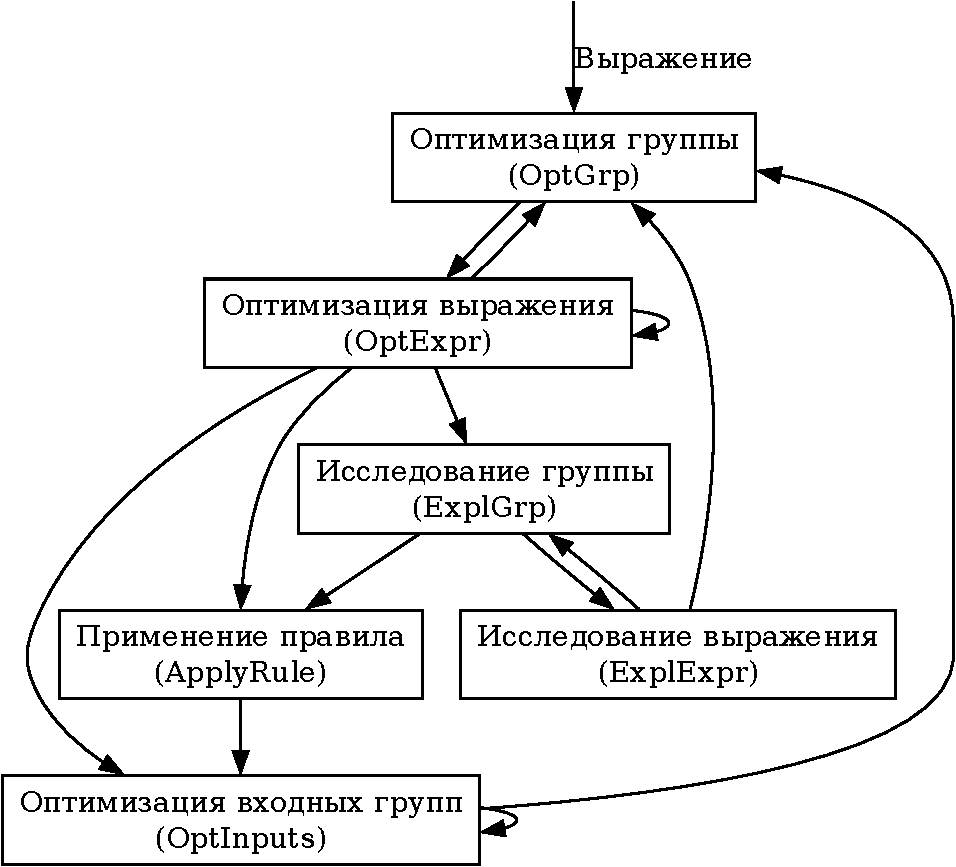
\includegraphics[width=0.8\textwidth]{cascades.pdf}
\caption{Схема взаимодействия задач в оптимизаторе Cascades}
\label{fig:cascades-tasks}
\end{figure}

\section{Правила трансформации и реализации}

Правило в оптимизаторе Cascades состоит из образца, условия применимости и
алгоритма применения. Образец описывает форму логического выражения, к которому
может быть применено правило. Условие применимости проверяет дополнительные
требования: отсутствие внешних ссылок, тип соединения, сохранение семантики
\texttt{NULL}, совместимость свойств и другие ограничения.

Формально правило можно представить как отображение:

\[
    r : pattern(e) \land condition(e) \rightarrow substitute(e),
\]

где \(e\) --- исходное выражение, \(pattern\) --- структурный образец,
\(condition\) --- предикат применимости, а \(substitute\) --- выражение-замена.
Для правил трансформации результатом применения является новое логическое
выражение в группе, а для правил реализации --- физическое выражение в той же
группе.

\subsection{Правила трансформации}

Правила трансформации применяются для исследования пространства эквивалентных
планов. Каждое из них задается тремя частями: паттерном, выражением-заменой и
условием активации.

Правило коммутативности соединения переставляет местами левый и правый входы
соединения. Эти преобразования позволяют оптимизатору рассмотреть оба порядка
вычисления и выбрать тот, при котором стоимость физического плана меньше.

\[
    R \bowtie_{\theta} S
    \Rightarrow
    S \bowtie_{\theta} R.
\]

Это правило применимо для внутренних и полных внешних соединений.

Правило ассоциативности соединения изменяет группировку цепочки соединений и
перераспределяет конъюнкты предикатов по ее узлам. Эти преобразования также
позволяют оптимизатору исследовать различные порядки выполнения соединений и
выбрать тот, при котором промежуточные результаты имеют наименьший размер.

\[
    (R \bowtie_{\theta_1} S) \bowtie_{\theta_2} T
    \Rightarrow
    R \bowtie_{\theta'_1} (S \bowtie_{\theta'_2} T),
\]

где \(\theta'_1\) и \(\theta'_2\) --- результат перераспределения конъюнктов
исходных предикатов \(\theta_1 \land \theta_2\) по тем узлам, в схемы которых
попадают все необходимые им атрибуты.

Условиями активации ассоциативности соединения являются:
\begin{itemize}
  \item оба соединения являются внутренними;
  \item конъюнкты предиката \(\theta_1 \land \theta_2\) можно перераспределить
        так, что атрибуты каждого конъюнкта в \(\theta'_2\) принадлежат
        \(attrs(S) \cup attrs(T)\), конъюнкты, ссылающиеся на \(attrs(R)\),
        остаются в \(\theta'_1\).
\end{itemize}

Правило проталкивания фильтрации через соединение перемещает фильтрующий
предикат над соединением в один из его входов. Эти преобразования позволяют
применить селективный предикат до соединения и тем самым уменьшить
кардинальность входа.

\[
    \sigma_p(R \bowtie_{\theta} S)
    \Rightarrow
    \sigma_p(R) \bowtie_{\theta} S,
    \quad attrs(p) \subseteq attrs(R),
\]

\[
    \sigma_p(R \bowtie_{\theta} S)
    \Rightarrow
    R \bowtie_{\theta} \sigma_p(S),
    \quad attrs(p) \subseteq attrs(S).
\]

Условиями активации проталкивания фильтрации через соединение являются:
\begin{itemize}
  \item атрибуты предиката \(p\) принадлежат только одному из входов соединения;
  \item соединение является внутренним, либо проталкивание выполняется в
        сохраняющий вход внешнего соединения.
\end{itemize}

Правило переноса фильтрации в предикат соединения объединяет фильтр над
соединением и предикат соединения в одно условие. Эти преобразования раскрывают
дополнительные равенства внутри предиката соединения, по которым физические
правила реализации могут построить эффективный алгоритм соединения, например
хеш-соединение или соединение слиянием.

\[
    \sigma_p(R \bowtie_{\theta} S)
    \Rightarrow
    R \bowtie_{\theta \land p} S.
\]

Частный случай для декартова произведения превращает его в полноценное
соединение с предикатом:

\[
    \sigma_p(R \times S)
    \Rightarrow
    R \bowtie_p S.
\]

Условиями активации переноса фильтрации в предикат соединения являются:
\begin{itemize}
  \item соединение является внутренним;
  \item атрибуты предиката \(p\) принадлежат \(attrs(R) \cup attrs(S)\).
\end{itemize}

Правило поднятия фильтрации над соединением переносит фильтр из одного из входов
соединения на уровень над самим соединением. Эти преобразования позволяют
объединить локальный фильтр с другими предикатами, расположенными выше по плану,
или открывают другие возможности применения правил.

\[
    \sigma_p(R) \bowtie_{\theta} S
    \Rightarrow
    \sigma_p(R \bowtie_{\theta} S),
    \quad attrs(p) \subseteq attrs(R).
\]

Условиями активации поднятия фильтрации над соединением являются:
\begin{itemize}
  \item атрибуты предиката \(p\) принадлежат только той ветви, из которой он
        поднимается;
  \item соединение является внутренним, либо подъем выполняется с сохраняющей
        стороны внешнего соединения.
\end{itemize}

Правило разбиения выборки на конъюнкты заменяет фильтр с конъюнктивным
предикатом на цепочку фильтров с отдельными подвыражениями. Эти преобразования
дают оптимизатору большую гранулярность для последующих трансформаций: каждый
конъюнкт может быть независимо протолкнут в нужную ветвь плана, переписан или
удален.

\[
    \sigma_{p_1 \land p_2 \land \ldots \land p_n}(R)
    \Rightarrow
    \sigma_{p_1}(\sigma_{p_2}(\ldots\sigma_{p_n}(R)\ldots)).
\]

Правило проталкивания проекции добавляет на каждый из входов соединения
проекцию, удаляющую атрибуты, не используемые ни предикатом соединения, ни
операторами выше по плану. Эти преобразования уменьшают ширину промежуточных
кортежей и сокращают объем данных, передаваемых между операторами.

\[
    \pi_L(R \bowtie_{\theta} S)
    \Rightarrow
    \pi_L\bigl(
        \pi_{L_R \cup J_R}(R)
        \bowtie_{\theta}
        \pi_{L_S \cup J_S}(S)
    \bigr),
\]

где \(L_R = L \cap attrs(R)\), \(L_S = L \cap attrs(S)\),
\(J_R = attrs(\theta) \cap attrs(R)\), \(J_S = attrs(\theta) \cap attrs(S)\).

Условием активации проталкивания проекции является нетривиальность хотя бы
одной из внутренних проекций: \(L_R \cup J_R \subsetneq attrs(R)\) или
\(L_S \cup J_S \subsetneq attrs(S)\). Иначе правило не уменьшает ширину
кортежей и его применение бесполезно.

Правило преобразования внешнего соединения во внутреннее заменяет левое и
правое, а также полное внешнее соединение на внутреннее соединение, если
расположенный над ними фильтр гарантированно отбрасывает все строки с
\texttt{NULL}-дополнением. Эти преобразования открывают для подплана с внешним
соединением правила, ограниченные внутренним соединением: коммутативность,
ассоциативность, проталкивание фильтрации и другие.

\[
    \sigma_p(R \operatorname{LOJ}_{\theta} S)
    \Rightarrow
    \sigma_p(R \bowtie_{\theta} S),
\]

\[
    \sigma_p(R \operatorname{ROJ}_{\theta} S)
    \Rightarrow
    \sigma_p(R \bowtie_{\theta} S),
\]

\[
    \sigma_p(R \operatorname{FOJ}_{\theta} S)
    \Rightarrow
    \sigma_p(R \bowtie_{\theta} S).
\]

Условиями активации преобразования внешнего соединения во внутреннее являются:
\begin{itemize}
  \item для левого внешнего соединения предикат \(p\) является
        null-отбрасывающим относительно атрибутов \(S\);
  \item для правого внешнего соединения предикат \(p\) является
        null-отбрасывающим относительно атрибутов \(R\);
  \item для полного внешнего соединения предикат \(p\) является
        null-отбрасывающим относительно атрибутов как \(R\), так и \(S\).
\end{itemize}

Null-отбрасывающим называется предикат, который при замене всех атрибутов
соответствующей стороны на \texttt{NULL} принимает значение, отличное от
\texttt{TRUE}.

Правило проталкивания агрегации ниже соединения добавляет частичную группировку
на одном из входов соединения, оставляя финальную комбинацию на верхнем уровне.
Эти преобразования уменьшают число строк, участвующих в соединении, и снимают
часть нагрузки с финальной агрегации.

\[
    \gamma_{G; F}(R \bowtie_{R.k = S.k} S)
    \Rightarrow
    \gamma_{G; F'}\bigl(
        \gamma_{G_R \cup \{R.k\}; F_R}^{partial}(R)
        \bowtie_{R.k = S.k}
        S
    \bigr),
\]

где \(G\) --- ключи группировки, \(F\) --- набор агрегатных функций,
\(G_R = G \cap attrs(R)\), \(F_R\) --- частичные агрегаты по атрибутам \(R\), а
\(F'\) --- финальные комбинаторы. Например, \texttt{SUM} раскладывается в сумму
частичных сумм, а \texttt{AVG} --- в пару \texttt{SUM} и \texttt{COUNT}.

Условиями активации проталкивания агрегации ниже соединения являются:
\begin{itemize}
  \item каждая агрегатная функция в \(F\) представима композицией частичной
        агрегации и финального комбинатора;
  \item соединение является внутренним эквивалентным соединением по
        \(R.k = S.k\);
  \item частичная агрегация группирует по объединению ключей группировки стороны
        \(R\) и ключа соединения \(R.k\).
\end{itemize}

Правило перестановки агрегации и соединения полностью выполняет агрегацию до
соединения. От проталкивания агрегации ниже соединения этот случай отличается
тем, что финальная комбинация после соединения не требуется. Это возможно
тогда, когда соединение не меняет результат агрегации: оно не дублирует и не
теряет строки агрегируемой стороны.

\[
    \gamma_{G; F_R}(R \bowtie_{R.k = S.k} S)
    \Rightarrow
    \gamma_{G; F_R}(R) \bowtie_{R.k = S.k} S.
\]

Условиями активации перестановки агрегации и соединения являются:
\begin{itemize}
  \item соединение является внутренним с предикатом равенства \(R.k = S.k\);
  \item агрегатные функции \(F_R\) вычисляются только по атрибутам \(R\), что
        позволяет выполнить агрегацию до того, как станут доступны атрибуты
        \(S\);
  \item каждой строке \(R\) при соединении соответствует ровно одна строка
        \(S\) с равным значением ключа, то есть \(S.k\) уникален и каждое
        значение \(R.k\) присутствует в \(S\). При нарушении уникальности
        соединение размножит строки \(R\), при нарушении ссылочной целостности
        часть строк \(R\) исчезнет;
  \item ключи группировки \(G\) содержат \(R.k\), то есть \(R.k \in G\).
        Без этого после агрегации значения \(R.k\) теряются и предикат
        соединения нельзя вычислить.
\end{itemize}

\subsection{Правила реализации}

Правила реализации переводят логические операторы в физические. Например, для
логического оператора чтения таблицы могут быть применены правила:

\begin{itemize}
  \item \texttt{LogicalGet} \(\Rightarrow\) \texttt{SeqScan};
  \item \texttt{LogicalGet} \(\Rightarrow\) \texttt{IndexScan}, если имеется
        индекс, совместимый с предикатом или требуемым порядком.
\end{itemize}

Для логического соединения могут быть созданы физические операторы
\texttt{NestedLoopJoin}, \texttt{HashJoin} и \texttt{MergeJoin}. Хеш-соединение
обычно требует предиката равенства по ключам, поскольку именно по ним строится
хеш-таблица. Сортировочное соединение требует, чтобы оба входа были
отсортированы по ключам соединения, либо чтобы оптимизатор мог добавить
сортировки как обеспечивающие операторы. Вложенные циклы применимы всегда, но
стоимость этого оператора может быть высокой без доступа к внутреннему отношению
с использованием индекса.

Правила реализации агрегации выбирают между хеш-агрегацией и потоковой
агрегацией. Хеш-агрегация не требует предварительного порядка, но потребляет
память пропорционально числу групп. Потоковая агрегация эффективна при уже
отсортированном входе, поскольку каждая группа обрабатывается последовательно.
Если требуемый порядок нужен также родительскому оператору, потоковая агрегация
может оказаться выгодной даже учитывая затраты на сортировку.

% {\color{red} TODO: псевдокод алгоритмов}

\subsection{Обеспечивающие операторы}

Физические свойства в Cascades обрабатываются через требуемые и предоставляемые
свойства. Если родительский оператор требует вход, отсортированный по атрибуту
\(a\), а выбранный дочерний план такого порядка не предоставляет, оптимизатор
может добавить обеспечивающий оператор \texttt{Sort}.

Обеспечивающие операторы не изменяют логический результат, но меняют физические
свойства и увеличивают стоимость. Поэтому они рассматриваются наравне с другими
физическими альтернативами. Например, план с хеш-соединением и последующей
сортировкой может конкурировать с планом на основе соединения слиянием, которое
сохраняет порядок результата.

\section{Метод ветвей и границ}

Метод ветвей и границ используется для сокращения пространства поиска и, как
следствие, неасимптотического улучшения скорости работы алгоритма. В контексте
Cascades ветвями являются альтернативные выражения и комбинации физических
реализаций дочерних групп, а границей является текущая лучшая стоимость плана
для заданной группы и требуемых физических свойств. Если нижняя оценка стоимости
частично построенного плана уже превышает текущую лучшую, дальнейшее
исследование по этой ветке не имеет смысла.

Пусть для группы \(G\) и требуемого свойства \(P\) уже найден план стоимости
\(C^*\). Рассматривается физическое выражение \(e\), имеющее локальную стоимость
\(C_{local}(e)\) и дочерние группы \(G_1, \ldots, G_k\). Если даже минимально
возможная оценка дочерних групп приводит к неравенству

\[
    C_{local}(e) + \sum_{i=1}^{k} LB(G_i, P_i) \geq C^*,
\]

то выражение \(e\) может быть отсечено. Здесь \(LB\) обозначает нижнюю границу
стоимости оптимизации дочерней группы под требуемым свойством \(P_i\). Чем
точнее нижняя граница, тем эффективнее отсечение.

На практике в качестве \(LB(G_i, P_i)\) принимается лучшая стоимость, найденная
для пары \((G_i, P_i)\) на текущий момент работы алгоритма. Поскольку
оптимизация группы является рекурсивным процессом, к моменту отсечения для
\((G_i, P_i)\) уже могут быть найдены некоторые планы, и их минимальная
стоимость служит нижней границей. Если же группа \(G_i\) под свойством \(P_i\)
ещё не рассматривалась, используется тривиальная граница \(LB = 0\), или, при
условии наличия минимальной стоимости на кортеж, можно принимать
\(LB(G_i, P_i) = |G_i| \cdot min_cost_per_row\).

Требуемые свойства дочерних групп \(P_i\) определяются оператором выражения \(e\)
совместно с требованием родителя \(P\). Каждый физический оператор описывает, какие
свойства он ожидает от своих входов: например, оператор сортирующего слияния требует
упорядоченности обоих входов по соответствующим ключам, тогда как хеш-соединение не
предъявляет требований к порядку. Таким образом, при спуске по дереву поиска каждый
оператор транслирует глобальное требование \(P\) в конкретные требования \(P_1,
\ldots, P_k\) к своим дочерним группам.

\subsection{Оценка кардинальности}

Оценка кардинальности является процессом предсказания числа кортежей,
возвращаемых оператором.

Для выборки используется селективность предиката \(sel(p)\), после чего
кардинальность результата оценивается как

\[
    |\sigma_p(R)| = |R| \cdot sel(p).
\]

Для соединения на основе предиката равенства независимых атрибутов часто
применяется эвристика:

\[
    |R \bowtie_{R.a = S.b} S| \approx
    \frac{|R| \cdot |S|}{\max(NDV(R.a), NDV(S.b))},
\]

где \(NDV\) --- число различных значений атрибута. Такая оценка удобна, но может
быть грубой, если данные имеют корреляции, сильный перекос или сложные
зависимости между атрибутами. Экспериментальные исследования показывают, что
ошибки кардинальности часто являются одной из основных причин выбора неудачных
планов~\cite{leis2015good}.

Для повышения качества оценок используются гистограммы, статистики по
многоколоночным ключам, сведения об уникальности, функциональные зависимости,
ограничения на схему, а в современных исследованиях также модели машинного
обучения.

\subsection{Оценка стоимости}

Функция стоимости сопоставляет физическому плану численную оценку затрат. В
простейшем случае стоимость можно представить как взвешенную сумму операций
чтения страниц, операций записи, вычислительных операций и сетевой передачи:

\[
    Cost(p) = w_{io} \cdot IO(p) + w_{cpu} \cdot CPU(p) +
              w_{mem} \cdot MEM(p) + w_{net} \cdot NET(p).
\]

Коэффициенты \(w_{io}\), \(w_{cpu}\), \(w_{mem}\) и \(w_{net}\) зависят от
конкретной аппаратной конфигурации.

Стоимость физического выражения обычно вычисляется рекурсивно:

\[
    Cost(node) = LocalCost(node) + \sum_{child \in children(node)} Cost(child).
\]

При этом локальная стоимость зависит от кардинальности входов и физических
свойств, а также конкретного физического оператора.

% {\color{red} TODO: табличка формул для разных операторов}

\section{Дифференциальный анализ физических планов}

Множество правил трансформации и реализации, используемых в
оптимизаторах запросов, изучено довольно хорошо и описано в
академической литературе. Вместе с тем условия активации правил
существенно различаются от системы к системе. Многие реализации
оптимизаторов упускают возможности для оптимизации из-за слишком
строгих условий активации правил или отсутствия определенных правил
в их наборе.

Данная проблема особенно актуальна при разработке нового оптимизатора: после
реализации базового набора правил возникает вопрос о полноте и корректности
этого набора по сравнению с устоявшимися и проверенными временем промышленными
системами. Такие системы аккумулировали обратную связь от пользователей и
уточняли условия активации своих правил в течение многих лет. Не имея такого
преимущества сложно добиться отличного качества построенных планов.

\subsection{Предлагаемый метод}

Для поиска несоответствий между поведением реализуемой системы и внешней
эталонной системы предлагается применить дифференциальный анализ планов.

Первым шагом нужно сформировать набор данных состоящий из схем таблиц и данных.
Далее, по заданным схемам генерируются случайные SQL-запросы различной структуры
и сложности. Такой подход исключает тривиальные планы и приближает условия
работы оптимизатора к реальным нагрузкам при дальнейшем построении планов
запросов.

Следующим шагом сгенерированные запросы транспилируются в диалекты SQL целевых
промышленных СУБД: Oracle, Microsoft SQL Server, PostgreSQL и т.д. Затем для
получения физических планов исполняется аналог \texttt{EXPLAIN ANALYZE}.

Полученные физические планы промышленных СУБД конвертируются в формат
сериализованного плана разрабатываемого оптимизатора. Для этого необходимо
создать набор отображений между физическими операторами различных систем.
Например, \texttt{Hash Match} в SQL Server отображается в \texttt{HashJoin} в
разрабатываемой системе, \texttt{Clustered Index Scan} --- в \texttt{IndexScan}
и так далее.

Корректность конвертации плана можно проверить путем исполнения исходого плана
на внешней системе и полученного плана на разрабатываемой системе и сравнения
полученных результатов.

Конвертированные планы сравниваются с планами, порождаемыми разрабатываемым
оптимизатором на исходных запросах, с целью определить, мог ли существующий
набор правил разрабатываемого оптимизатора породить план, эквивалентный плану
промышленной системы. Для корректности сравнения необходимо полное исследование
пространства эквивалентных планов. Если разрабатываемая система не может
породить ``эталонный'' план, то условия активации или набор правил требует
уточнения. Определение требуемых изменений лежит на разработчике системы,
поэтому найденный запрос и примеры планов сохраняются для последующего анализа.
В дальнейшем, полученные после конвертации ``эталонные'' планы можно
использовать как тесты для оптимизатора, которые будут успешно выполняться после
уточнения соответвующих правил активации.

\subsection{Поиск ближайшего плана}

В случае невозможности построить ``эталонный'' план разрабатываемым
оптимизатором, предлагается искать ближайший план, т.е. план из пространства
поиска разрабатываемого оптимизатора, максимально близкий к плану промышленной
системы. При этом метрика расстояния между планами может быть определена как
расстояние редактирования деревьев.

Анализ ближайшего плана может помочь упростить выявление трансформаций, которые
разрабатываемый план по какой-то причине не применил.

\subsection{Область применения}

Предлагаемый метод дифференциального анализа применим не только для сравнения с
проприетарными системами, но и с СУБД с открытым исходным кодом, позволяя
уточнять условия применения правил.

Систематическое применение этого подхода позволяет построить итеративный процесс
совершенствования оптимизатора:

\begin{itemize}
  \item генерация запросов;
  \item запуск и сбор планов;
  \item приведение к единому виду, сравнение и выявление расхождений;
  \item добавление или корректировка правил;
  \item повторное сравнение.
\end{itemize}

Таким образом, дифференциальный анализ обеспечивает управляемое и измеримое
улучшение качества оптимизатора и позволяет новым или открытым оптимизаторам
быстрее достигать качества устоявшихся промышленных оптимизаторов.

% {\color{red} TODO: описать как нормализовать и т.п.}

\renewcommand\refname{СПИСОК ИСПОЛЬЗОВАННЫХ ИСТОЧНИКОВ}
\clearpage
{\catcode`"\active\def"{\relax}
    \addcontentsline{toc}{section}{\protect\numberline{}\refname}%
    \printbibliography
}
\newpage

\settocdepth{section}
\anonsection{ПРИЛОЖЕНИЕ А}
\vspace{-30pt}

\begin{algorithm}[H]
    \caption{Алгоритм поиска (часть 1).}
    \label{alg:cascades-search}
    \begin{algorithmic}[1]

    \Procedure{Optimize}{$root$}
        \State Push task $\Call{OptimizeGroup}{root.group, \bot}$ onto task stack
        \While{task stack is not empty}
            \State Pop and execute next task
        \EndWhile
        \State \Return $best\_plan[root.group]$
    \EndProcedure

    \Procedure{OptimizeGroup}{$group, limit$}
        \If{$best\_cost[group]$ exists \textbf{and} ($limit = \bot$ \textbf{or} $best\_cost[group] < limit$)}
            \State \Return
        \EndIf
        \If{$group$ is not explored}
            \State Push task $\Call{OptimizeGroup}{group, limit}$ onto task stack
            \State Push task $\Call{ExploreGroup}{group, limit}$ onto task stack
            \State \Return
        \EndIf
        \For{each logical expression $expr \in group$}
            \State Push task $\Call{OptimizeExpression}{expr, limit}$ onto task stack
        \EndFor
    \EndProcedure

    \Procedure{ExploreGroup}{$group, limit$}
        \State Mark $group$ as explored
        \For{each logical expression $expr \in group$}
            \State Push task $\Call{ExploreExpression}{expr, limit}$ onto task stack
        \EndFor
    \EndProcedure
    \end{algorithmic}
\end{algorithm}

\begin{algorithm}[H]
    \caption{Алгоритм поиска (часть 2).}
    \label{alg:cascades-search-2}
    \begin{algorithmic}[1]
    \Procedure{ExploreExpression}{$expr, limit$}
        \For{each applicable transformation rule $r$}
            \State Push task $\Call{ApplyTransformation}{r, expr, limit}$ onto task stack
        \EndFor
        \For{each child group $child \in \Call{Children}{expr}$}
            \If{$child$ is not explored}
                \State Push task $\Call{ExploreGroup}{child, limit}$ onto task stack
            \EndIf
        \EndFor
    \EndProcedure

    \Procedure{OptimizeExpression}{$expr, limit$}
        \For{each applicable implementation rule $r$}
            \State Push task $\Call{ApplyImplementation}{r, expr, limit}$ onto task stack
        \EndFor
        \For{each child group $child \in \Call{Children}{expr}$}
            \If{$child$ is not explored}
                \State Push task $\Call{ExploreGroup}{child, limit}$ onto task stack
            \EndIf
        \EndFor
    \EndProcedure

    \Procedure{ApplyTransformation}{$rule, expr, limit$}
        \State $new\_expr \leftarrow \Call{Apply}{rule, expr}$
        \State Push task $\Call{ExploreExpression}{new\_expr, limit}$ onto task stack
    \EndProcedure

    \Procedure{ApplyImplementation}{$rule, expr, limit$}
        \State $phys \leftarrow \Call{Apply}{rule, expr}$
        \State $lc \leftarrow \Call{CalcLocalCost}{phys}$
        \If{$limit \neq \bot$ \textbf{and} $lc \geq limit$}
            \State \Return
        \EndIf
        \State $child\_limit \leftarrow (limit = \bot) \mathbin{?} \bot \mathbin{:} limit - lc$
        \State Push task $\Call{OptimizeInputs}{phys, child\_limit, 0}$ onto task stack
    \EndProcedure
    \end{algorithmic}
\end{algorithm}

\begin{algorithm}[H]
    \caption{Алгоритм поиска (часть 3).}
    \label{alg:cascades-search-3}
    \begin{algorithmic}[1]
    \Procedure{OptimizeInputs}{$expr, limit, i$}
        \State $children \leftarrow \Call{Children}{expr}$
        \If{$i \geq |children|$}
            \State $total \leftarrow local\_cost[expr] + accum\_child\_cost[expr]$
            \If{$best\_cost[expr.group]$ does not exist \textbf{or} $total < best\_cost[expr.group]$}
                \State $best\_cost[expr.group] \leftarrow total$
                \State $best\_plan[expr.group] \leftarrow expr$
            \EndIf
            \State \Return
        \EndIf
        \State $child \leftarrow children[i]$
        \State Push task: \textbf{if} $best\_cost[child]$ exists \textbf{then} accumulate child cost \textbf{and} push $\Call{OptimizeInputs}{expr, \ldots, i+1}$
        \State Push task $\Call{OptimizeGroup}{child, limit}$ onto task stack
    \EndProcedure
    \end{algorithmic}
\end{algorithm}

\end{document}
